% ACL 2026 long paper (ARR). Compile with pdfLaTeX + BibTeX:
%   latexmk -pdf main.tex      (or Overleaf: upload this whole folder)
% Red \todo{...} marks writing that is still missing; red \tbd cells mark results not yet in.
% Every number comes from SkillParseUMR/experiment/orchestration-v2 (results/summary.json).
\documentclass[11pt]{article}
\usepackage[review]{acl}
\usepackage{times}
\usepackage{latexsym}
\usepackage[T1]{fontenc}
\usepackage[utf8]{inputenc}
\usepackage{microtype}
\usepackage{inconsolata}
\usepackage{graphicx}
\usepackage{amsmath}
\usepackage{amssymb}
\usepackage{booktabs}
\usepackage{multirow}
\usepackage{enumitem}
\usepackage{xspace}
\usepackage{xcolor}
\usepackage{CJKutf8}
\usepackage{tikz}
\usepackage{algorithm}
\usepackage{algpseudocode}
\usepackage[safe]{tipa}
\usetikzlibrary{positioning,arrows.meta,fit,backgrounds,calc}

% ---------------------------------------------------------------- macros
\newcommand{\umr}{\textsc{UMR}\xspace}
\newcommand{\amr}{\textsc{AMR}\xspace}
\newcommand{\ours}{decision orchestration\xspace}
\newcommand{\Ours}{Decision orchestration\xspace}
\newcommand{\skill}[1]{\texttt{#1}}
\newcommand{\zh}[1]{\begin{CJK}{UTF8}{gbsn}#1\end{CJK}}
\newcommand{\zht}[1]{\begin{CJK}{UTF8}{bsmi}#1\end{CJK}}   % traditional characters (PARSEME Chinese)
\newcommand{\todo}[1]{\textcolor{red}{[TODO: #1]}}
\newcommand{\tbd}{\textcolor{red}{--}}
\newcommand{\exper}[1]{\textcolor{red}{\textsc{[#1]}}}   % pointer to an experiment in PLAN.md
\newcommand{\F}{F\xspace}
\newcommand{\jm}{\textipa{ju:m\ae tS}}   % the official UMR shared-task metric

% ---------------------------------------------------------------- float spacing (tighter than the defaults)
\setlength{\textfloatsep}{10pt plus 2pt minus 3pt}
\setlength{\dbltextfloatsep}{10pt plus 2pt minus 3pt}
\setlength{\floatsep}{8pt plus 2pt minus 2pt}
\setlength{\dblfloatsep}{8pt plus 2pt minus 2pt}
\setlength{\abovecaptionskip}{5pt}
\renewcommand{\topfraction}{0.9}
\renewcommand{\dbltopfraction}{0.9}
\renewcommand{\textfraction}{0.07}
\renewcommand{\floatpagefraction}{0.85}

\title{Don't Read the Whole Guideline: Decision Orchestration for\\
Complex Annotation with Small Models and Little Supervision}

\author{Anonymous ACL submission}

\begin{document}
\maketitle

\begin{abstract}
A new annotation scheme, language or domain usually starts with a guideline and little annotated data. We propose \emph{decision orchestration}: the guideline is written as an executable procedure in which rules enumerate candidates and assemble the output, and a decision model answers only closed questions, returning a probability for each option the guideline allows. The output is well-formed by construction, every decision is cheap and has a confidence, and uncertain decisions can be routed to a stronger model. We learn the procedure, not model weights: an LLM reflector reads five annotated sentences at a time, with the gold and predicted annotations and every question asked, and proposes edits to the procedure's rules, options and thresholds; each edit is kept only if it measurably improves the score. On verbal multiword expression identification (PARSEME), a procedure learned from 60 annotated sentences reaches 46.3 F in English, 13 points above the best system of the 2018 shared task, which was trained on 3,471 sentences, and 57.8 F in Chinese, 18 points above an LLM annotating directly with ten gold examples; reflection costs under one dollar per language. On Uniform Meaning Representation parsing, where the output is mostly graph structure, closed decisions alone do not beat direct generation, although reflection adapts a Chinese procedure to English (+4.1 F) and routing adds 2.5 F. Decision orchestration pays off where a guideline is a sequence of tests over enumerable candidates.
\end{abstract}

%=====================================================================
\section{Introduction}
\label{sec:intro}

\begin{figure*}[t]
\centering
\resizebox{\textwidth}{!}{%
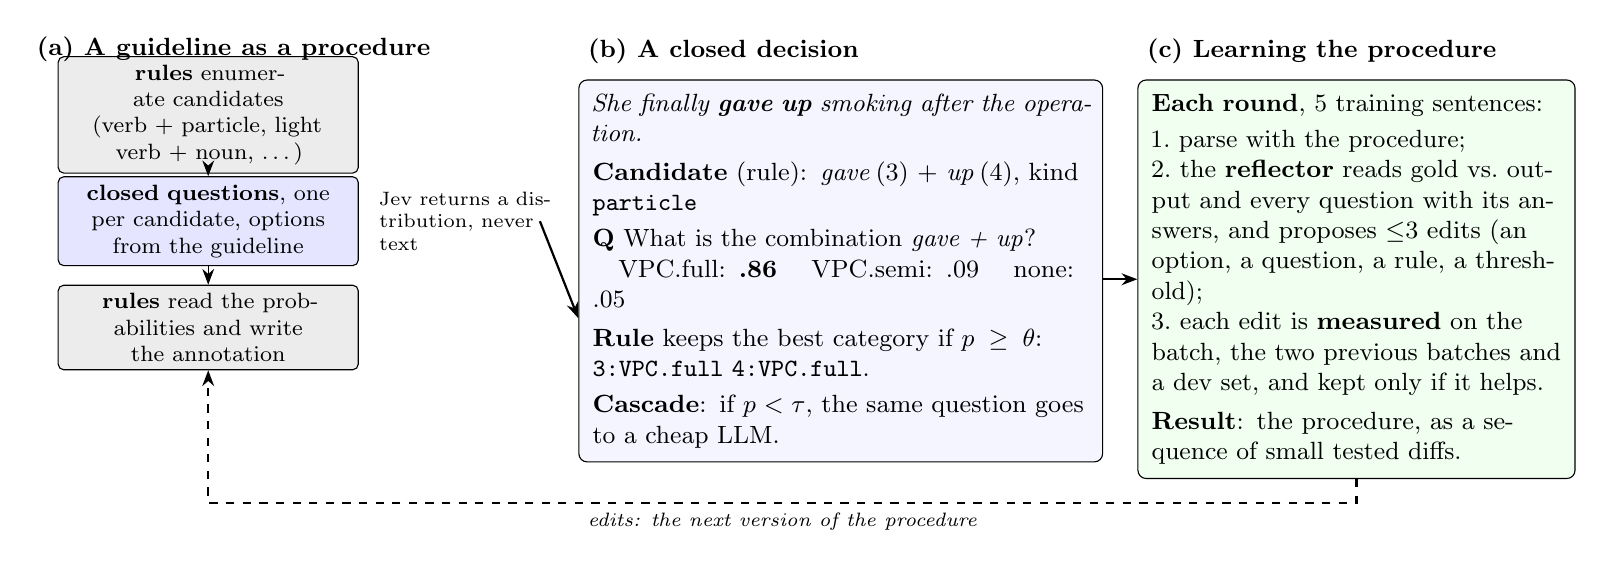
\begin{tikzpicture}[
    font=\small,
    >={Stealth[length=2mm]},
    rule/.style={draw, rounded corners=2pt, fill=gray!15, minimum height=6mm, inner sep=3pt, align=center, font=\footnotesize},
    dec/.style={draw, rounded corners=2pt, fill=blue!10, minimum height=6mm, inner sep=3pt, align=center, font=\footnotesize},
    box/.style={draw, rounded corners=3pt, inner sep=5pt, align=left},
    ttl/.style={font=\small\bfseries, anchor=south west},
  ]
  % ---------------- (a) the procedure
  \node[rule, text width=3.6cm] (cand) at (2.2,0) {\textbf{rules} enumerate candidates\\(verb + particle, light verb + noun, \dots)};
  \node[dec, text width=3.6cm] (ask) at (2.2,-1.35) {\textbf{closed questions}, one per candidate, options from the guideline};
  \node[rule, text width=3.6cm] (asm) at (2.2,-2.7) {\textbf{rules} read the probabilities and write the annotation};
  \draw[->] (cand) -- (ask); \draw[->] (ask) -- (asm);
  \node[font=\scriptsize, anchor=west, text width=2.3cm] at (4.25,-1.35) {Jev returns a distribution, never text};
  \node[ttl] at (-0.1,0.55) {(a) A guideline as a procedure};
  % ---------------- (b) a closed decision
  \node[box, fill=blue!4, text width=6.3cm, anchor=north west] (q) at (6.9,0.45) {%
    \emph{She finally \textbf{gave up} smoking after the operation.}\\[3pt]
    \textbf{Candidate} (rule): \emph{gave}\,(3) + \emph{up}\,(4), kind \texttt{particle}\\[2pt]
    \textbf{Q} What is the combination \emph{gave + up}?\\
    \quad VPC.full: \textbf{.86} \quad VPC.semi: .09 \quad none: .05\\[3pt]
    \textbf{Rule} keeps the best category if $p \geq \theta$: \texttt{3:VPC.full 4:VPC.full}.\\[2pt]
    \textbf{Cascade}: if $p < \tau$, the same question goes to a cheap LLM.};
  \node[ttl] at ([yshift=2pt]q.north west) {(b) A closed decision};
  % ---------------- (c) learning in batches
  \node[box, fill=green!6, text width=5.2cm, anchor=north west] (l) at (14.0,0.45) {%
    \textbf{Each round}, 5 training sentences:\\[2pt]
    1.~parse with the procedure;\\
    2.~the \textbf{reflector} reads gold vs.\ output and every question with its answers, and proposes $\leq$3 edits (an option, a question, a rule, a threshold);\\
    3.~each edit is \textbf{measured} on the batch, the two previous batches and a dev set, and kept only if it helps.\\[3pt]
    \textbf{Result}: the procedure, as a sequence of small tested diffs.};
  \node[ttl] at ([yshift=2pt]l.north west) {(c) Learning the procedure};
  \draw[->, thick] (ask.east) ++(2.3,0) -- ([yshift=-6mm]q.west);
  \draw[->, thick] (q.east |- l.west) -- (l.west);
  \coordinate (low) at ([yshift=-3mm]l.south);
  \draw[->, thick, dashed] (l.south) -- (low) -| node[font=\scriptsize\itshape, pos=0.25, below] {edits: the next version of the procedure} (asm.south);
\end{tikzpicture}}
\caption{Decision orchestration. (a)~A guideline is written as a procedure in which rules enumerate candidates and assemble the output, and a decision model answers closed questions with probabilities. (b)~One closed decision in the verbal-multiword-expression procedure. (c)~The procedure is learned from a few annotated sentences at a time: an LLM proposes edits, and each edit is kept only if it measurably helps.}
\label{fig:overview}
\end{figure*}

A new annotation scheme, or an old one in a new language or domain, usually starts with a written guideline and very little annotated data. Training a supervised model needs thousands of examples; prompting an LLM to write the annotation needs none, but hands the model the whole job: deciding what to annotate, applying the scheme's conventions, and producing well-formed output, all at once and at the price of a generative model for every sentence.

Most of a guideline is not judgment. It tells the annotator where to look, which units to consider, which tests to apply in which order, and how to write the result; only some steps require understanding the sentence. We propose \textbf{decision orchestration} (Figure~\ref{fig:overview}): write the guideline as an executable \emph{procedure} in which rules enumerate candidates and assemble the output, and a \emph{decision model} answers only closed questions, each a choice among options taken from the guideline, with a probability distribution. The output is well-formed by construction. Every decision is cheap, inspectable and comes with a confidence. Uncertain decisions can be routed to a stronger model.

A hand-written procedure encodes the guideline as its author read it. Gold annotations encode the conventions annotators actually followed, and the two differ. We therefore \emph{learn the procedure}, not model weights. An LLM reflector reads five training sentences at a time, with the gold and predicted annotations and every question asked with its answer, and proposes small edits to the procedure's code, options and thresholds. Each edit is kept only if it improves the score on the batch, on earlier batches and on a development set. The procedure's history becomes a sequence of small tested diffs that a person can read, and the whole learning process costs a few dollars.

We test the method on two schemes that differ in how much of the output is structure: verbal multiword expressions (PARSEME), where an annotation is a set of categorized token groups, and Uniform Meaning Representation (UMR), where it is a graph. Each is tested in Chinese and English. Our findings:
\begin{itemize}[leftmargin=*,itemsep=2pt,topsep=2pt]
\item On PARSEME, a procedure learned from \textbf{60 annotated sentences} reaches 46.3 F on English, \textbf{13 points above the best system of the 2018 shared task}, which trained on all 3,471 training sentences, and 57.8 F on Chinese, \textbf{18 points above} Claude Haiku annotating directly with ten gold examples. Twelve rounds of reflection add 5.5 F on Chinese (7.8 on unseen expressions) for \$0.53 of reflector calls, and the decisions for the whole Chinese test set cost \$0.06.
\item On UMR, where the output is mostly structure, closed decisions alone do not beat direct generation. Routing uncertain decisions adds 2.5 F in Chinese, and reflection adapts a procedure written for Chinese to English (+4.1 F); but direct generation with ten examples matches the best procedure in Chinese and exceeds it by 16 F in English.
\item The procedure's options must follow the annotation's conventions, not the full inventory of the guideline: a UMR procedure that offered the decision model the 27-value aspect lattice of the guidelines, where the gold uses seven coarse values, gained 5.2 F when its aspect options were restricted to those seven and one polarity rule was restored.
\end{itemize}
Decision orchestration thus pays off where a guideline is a sequence of tests over enumerable candidates, and it tells us, through the measured edits and the routed decisions, where a scheme is not.

%=====================================================================
\section{Related Work}
\label{sec:related}

\paragraph{LLMs as annotators.}
LLMs can label data directly \citep{wang2021reduce,gilardi2023chatgpt,he2024annollm,ziems2024css,tan2024annotation}, and human--LLM collaboration routes uncertain items to people \citep{li2023coannotating,wang2024humanllm}. GoLLIE \citep{sainz2024gollie} fine-tunes a model to follow guidelines written as code, Code4Struct \citep{wang2023code4struct} writes event structures as code, and guideline learning \citep{pang2023guideline} induces guideline text from errors. These keep the model in charge of writing the annotation. We keep the guideline's procedure in code and ask the model only closed questions inside it, so the output is well-formed by construction and every decision has a probability.

\paragraph{LM programs and structured output.}
Prompt chains and decomposed prompting compose model calls \citep{wu2022aichains,khot2023decomposed}; programs can call models or declare their constraints \citep{gao2023pal,gupta2023visprog,beurer2023lmql,khattab2024dspy}, and grammar-constrained decoding controls output form \citep{willard2023outlines,geng2023grammar}, possibly at a cost to reasoning \citep{tam2024speak}. Agents let the model choose the next step \citep{yao2023react}. In our procedures the control flow is fixed code, and the model's only output is a distribution over listed options.

\paragraph{Optimizing prompts and programs.}
Prompts and programs can be optimized from feedback \citep{zhou2023ape,pryzant2023protegi,yang2024opro,opsahl2024mipro,yuksekgonul2025textgrad}, by reflecting on execution traces \citep{agrawal2025gepa} or by growing a playbook of lessons \citep{zhang2025ace}; workflows and scaffolds can be searched as well \citep{zhang2025aflow,hu2025adas,zelikman2024stop}. Self-feedback without an external signal is unreliable \citep{huang2024cannot}. Our reflector reads gold-aligned traces of a few sentences and edits code, options and thresholds; every edit is kept only if it measurably helps. The result resembles transformation-based learning \citep{brill1995transformation} and data programming \citep{ratner2017snorkel} in being a readable artifact, but its rules are written by an LLM and checked by measurement.

\paragraph{Calibration and cascades.}
Calibration and selective prediction study when to trust a model's confidence \citep{guo2017calibration,jiang2021calibration,zhao2021calibrate,kamath2020selective,kadavath2022know}; cascades escalate inputs to costlier models \citep{chen2023frugalgpt}. We escalate individual closed questions inside a structured annotation, by the decision model's own probability.

\paragraph{The two tasks.}
PARSEME systems for verbal multiword expressions are mostly supervised sequence taggers or graph-based parsers trained on the full training data, often on top of pretrained encoders \citep{ramisch2018parseme,ramisch2020parseme}; the 2.0 edition also reports instruction-tuned LLMs \citep{scholivet2026parseme}. Meaning representation parsers likewise learn from large corpora \citep{bevilacqua2021spring,zhou2021structure,bai2022graph}, which \umr does not yet have \citep{gysel2021design,bonn2023umr,bonn2024infrastructure,bonn2025umr2}; \citet{chun2024pipeline} convert other representations, and \citet{markle2025setup} propose a parsing setup for \umr. We use both tasks as tests of a method for learning annotation procedures from little data, not to compete with systems trained on full corpora.

%=====================================================================
\section{Decision Orchestration}
\label{sec:method}

\paragraph{Setting.}
An annotation scheme maps an input $x$ (a sentence, or a document) to a structured annotation $y$: a set of typed token groups, a graph, a set of relations. In the cold start we have the scheme's prose guideline, the external resources it refers to (e.g., a frame lexicon), an automatic scorer, and a few annotated sentences. We train no model weights. We write, and then learn, a \emph{procedure} $\Pi$ that maps $x$ to $y$.

\subsection{Procedures: rules around closed decisions}
\label{sec:procedure}
A guideline is mostly a procedure: it says where to look, which units to consider, which tests to apply in which order, and how to write the result. Only some steps need judgment. $\Pi$ makes this split explicit (Figure~\ref{fig:overview}). It consists of three parts.
\begin{itemize}[leftmargin=*,itemsep=1pt,topsep=2pt]
\item \textbf{Rules} enumerate candidates from the input (words, spans, verb--object pairs, the senses of a verb in a lexicon, the mentions before a pronoun) and decide what is decidable without judgment (number formats, function words, the assembly of the output).
\item \textbf{Closed questions} cover the rest. A question names its subject in the input and lists its options, each with a one-line description taken from the guideline: a choice (``which category is \emph{give up} here: VPC.full, VPC.semi, none''), a yes/no question, or a graded score. Questions are asked in rounds; a round may depend on the answers of the previous one.
\item \textbf{Parameters} $\theta$, such as the probability an option needs before a rule acts on it.
\end{itemize}
A decision model answers every question of a round at once with a probability distribution over its options and no text. Rules read the distributions against $\theta$ and assemble $y$. The output is well-formed by construction, since only rules write it, and every decision carries a probability that can be inspected, thresholded or routed. In our implementation a procedure is a folder of Python files with their question texts and option lists, which makes it readable and editable by a person and by a language model alike.

\paragraph{Decision model.}
We use Jev \citep{typesafe2026jev}, a model served behind a typed closed-question interface (choice, yes/no, score) that returns only probabilities. The interface fixes what the model can do: it never writes structure, so a procedure is the only place where the annotation's form is defined. Decisions are cheap. At the list price we used, \$0.02 per million tokens, a decision costs a few hundred-thousandths of a dollar. Answers are cached by request, so re-running a procedure only pays for the questions that changed.

\subsection{Learning the procedure in small batches}
\label{sec:reflection}
A hand-written procedure encodes the guideline as its author read it; the gold data encode the conventions annotators actually followed. We close the gap by editing the procedure, never model weights, a few sentences at a time (Algorithm~\ref{alg:reflect}). Each round $r$ takes the next batch $B_r$ of five training sentences and parses it with the current procedure. A \emph{reflector}, a general LLM (Claude Sonnet 5.5), reads a report of the batch: the gold and predicted annotations, the scorer's findings, and, for every node, the questions asked and the distributions Jev returned. It sees the procedure's editable files and the titles of edits tried in earlier rounds, diagnoses the most costly differences and proposes at most three edits, each an exact find-and-replace in one file: a new option with the rule branch that uses it, a new question where a rule guessed, a changed threshold, a convention written into a rule, or a clarified option description.

Every edit is \emph{measured} before it is kept. It is applied on top of the edits already accepted in the round, and the procedure is re-run on three sets: the batch, a regression set (the batches of the two previous rounds) and a fixed development set. The edit stays if the mean $F$ over the three rises by at least 0.3, development $F$ does not fall by more than 0.5, regression $F$ by no more than 1.0, and no new runtime errors appear. Rejected edits go back to the reflector once, with their measured effect on each set, to be narrowed or rewritten. Because Jev's answers are cached, a trial pays only for the questions that the edit changes; a whole round costs cents in decisions and a few cents in reflector calls.

Small batches keep the reflector's context short and its diagnosis specific, and they make the procedure's history a sequence of small, attributable, tested changes. The regression and development sets keep the procedure from overfitting to the batch; we find that a development set of ten sentences is too small to do so reliably (\S\ref{sec:analysis}).

\begin{algorithm}[t]
\small
\caption{Measured reflection in small batches.}
\label{alg:reflect}
\begin{algorithmic}[1]
\Require seed procedure $\Pi_0$, training pool $P$, development set $D$, batch size $b{=}5$
\For{$r = 1, \dots, R$}
  \State $B \gets$ next $b$ sentences of $P$; $G \gets$ batches of rounds $r{-}2, r{-}1$
  \State $s \gets \textsc{Score}(\Pi, \{B, G, D\})$
  \State $E \gets \textsc{Reflect}(\Pi, \textsc{Report}(\Pi, B))$ \Comment{$\leq 3$ edits}
  \For{$e \in E \cup \textsc{Revise}(\text{rejected})$}
    \State $s' \gets \textsc{Score}(e(\Pi), \{B, G, D\})$
    \If{$\bar{s}' - \bar{s} \geq 0.3 \wedge s'_D - s_D \geq -0.5 \wedge s'_G - s_G \geq -1$}
      \State $\Pi \gets e(\Pi)$; $s \gets s'$
    \EndIf
  \EndFor
\EndFor
\end{algorithmic}
\end{algorithm}

\subsection{Routing uncertain decisions}
\label{sec:cascade}
Each decision comes with a probability, so the procedure knows which of its decisions are uncertain. In the \emph{cascade}, a question whose top option has probability below $\tau$ is asked again of a cheap generative model (Claude Haiku 5.5), given the same input and the same question and options; its answer replaces Jev's. The procedure itself is unchanged, and only uncertain questions pay the higher price.

%=====================================================================
\section{Experimental Setup}
\label{sec:setup}

\paragraph{Models.}
Closed decisions are answered by Jev (\texttt{jev-1.13-20260917}) through OpenRouter. The reflector is Claude Sonnet 5.5 and the cascade model Claude Haiku 5.5, both through OpenRouter at temperature 0 (0.3 when the reflector's first reply cannot be parsed). We report the costs that the service billed for each request.

\paragraph{Reflection.}
Every run has twelve rounds of five training sentences (60 sentences in all). The reflector proposes at most three edits per round and may rewrite the rejected ones once. An edit is kept under the measured criterion of \S\ref{sec:reflection}. Before an edit is tried, it is checked for text copied from the test sentences (six consecutive Chinese characters or four English words); none was found. The development and test sets are never shown to the reflector. Seeds and every round's version are frozen, and all reported test runs use a version that existed before any test sentence was parsed with it.

\paragraph{Baselines.}
(i)~\emph{Direct generation}: Claude Haiku 5.5 writes the annotation itself, one call per sentence, given the scheme's category or concept inventory and the first ten sentences of the reflection pool with their gold annotation; it thus sees one sixth of the gold that reflection reads, in full, at every call. (ii)~For PARSEME, the systems of the shared tasks, trained on the full training data and in the open track on pretrained models, re-scored from their released test predictions with the official script and the same training file. (iii)~For Chinese \umr, two closed procedures from earlier work on these data: the seed J2 and K4, the latter after four rounds of document-level measured reflection with a different reflector (seven training documents in all).

\paragraph{Metrics.}
PARSEME: the official MWE-based F1 (exact token set and category) and its restriction to VMWEs unseen in the training file. \umr: AnCast++ sentence-graph F; each test document is scored on its sentences with gold, and we average over documents. In a pilot on these data, a cold re-run of the same Jev procedure changed a document's \umr F by at most about 0.6; we treat smaller differences as noise.

%=====================================================================
\section{Results}
\label{sec:results}

\begin{table*}[t]
\centering\small
\setlength{\tabcolsep}{5pt}
\begin{tabular}{@{}llrcccc@{}}
\toprule
& & \multicolumn{1}{c}{training} & \multicolumn{2}{c}{Chinese (1.2)} & \multicolumn{2}{c}{English (1.1)} \\
\cmidrule(lr){4-5}\cmidrule(lr){6-7}
System & & \multicolumn{1}{c}{sentences} & F & unseen F & F & unseen F \\
\midrule
\multicolumn{7}{@{}l}{\emph{Shared-task systems, trained on the full training data (re-scored)}} \\
\quad best open track & & all & 71.9 & 64.2 & 33.3 & 23.7 \\
\quad best closed track & & all & 60.9 & 45.7 & 32.9 & 17.6 \\
\midrule
\multicolumn{7}{@{}l}{\emph{Direct generation}} \\
\quad Claude Haiku 5.5, 10 gold examples & & 10 & 39.5 & 32.6 & 41.1 & 34.8 \\
\midrule
\multicolumn{7}{@{}l}{\emph{Decision orchestration (Jev decisions)}} \\
\quad seed procedure & $\Pi_0$ & 0 & 52.4 & 36.5 & 44.3 & 37.8 \\
\quad after 6 rounds & $\Pi_6$ & 30 & 56.9 & 43.1 & \textbf{46.3} & \textbf{38.8} \\
\quad after 12 rounds & $\Pi_{12}$ & 60 & 57.8 & 44.3 & \textbf{46.3} & \textbf{38.8} \\
\quad $\Pi_{12}$ + Haiku cascade ($\tau{=}0.7$) & & 60 & \textbf{58.5} & \textbf{45.7} & 44.1 & 37.4 \\
\bottomrule
\end{tabular}
\caption{PARSEME test sets: MWE-based F1 and F1 on VMWEs unseen in the training file, all computed with the official script from the systems' released predictions. Best open track: TRAVIS-mono (Chinese), Milos (English); best closed track: ERMI, TRAPACC. ``Training sentences'' are the annotated sentences a system used; the reflector read five per round.}
\label{tab:parseme}
\end{table*}

\paragraph{Learned procedures beat direct generation on PARSEME.}
Table~\ref{tab:parseme} gives the PARSEME results. The seed procedures, written from the guidelines before any training sentence was read, already exceed direct generation with ten gold examples: 52.4 vs.\ 39.5 F in Chinese and 44.3 vs.\ 41.1 in English. Reflection adds 5.5 F in Chinese (7.8 on unseen expressions) and 2.0 in English. In English, the learned procedure scores 13 points above the best system of the 2018 shared task, which was trained on all 3,471 training sentences. Those systems predate today's pretrained encoders, so the comparison shows how little data the procedure needs rather than a new state of the art. In Chinese, the open-track systems trained on 35,326 sentences on top of multilingual pretrained encoders remain 14 points ahead, and the procedure is 3 points below the best closed-track system. Precision is the weak side of both procedures: the final Chinese procedure finds 71\% of the gold VMWEs, but only 49\% of its predictions are correct.

\paragraph{Routing helps where Jev is unsure and the cheap model is right.}
In Chinese, the cascade re-asked 361 questions (\$0.09) and gained 0.7 F (1.4 on unseen expressions). In English it re-asked 720 questions and lost 2.2 F: Haiku accepted 123 more candidates as VMWEs, of which 13 were correct. Whether to route is an empirical question per task, which a development set can answer before deployment.

\begin{table}[t]
\centering\small
\setlength{\tabcolsep}{4pt}
\begin{tabular}{@{}lcc@{}}
\toprule
System & zh & en \\
\midrule
Haiku 5.5, 10 gold examples & 42.0 & \textbf{46.4} \\
\midrule
\multicolumn{3}{@{}l}{\emph{Chinese procedures of earlier work}} \\
\quad J2 (seed) & 39.4 & -- \\
\quad K4 (J2 + 4 document rounds) & 40.1 & -- \\
\quad K4 + Haiku cascade, $\tau{=}0.7$ & \textbf{42.6} & -- \\
\quad K4 + Haiku cascade, $\tau{=}0.9$ & 41.6 & -- \\
\midrule
\multicolumn{3}{@{}l}{\emph{Revised procedure (questions in data files)}} \\
\quad as released (27 aspect values) & 33.3 & -- \\
\quad $\Pi_0$: + aspect / polarity conventions & 38.5 & 26.0 \\
\quad $\Pi_6$ & 38.2 & 29.7 \\
\quad $\Pi_{12}$ & 38.2 & 30.1 \\
\quad $\Pi_{12}$ + Haiku cascade, $\tau{=}0.7$ & -- & 30.5 \\
\bottomrule
\end{tabular}
\caption{\umr test sets: AnCast++ sentence F, macro-averaged over documents (Chinese: 8 documents, 138 sentences; English: 6, 143). The English procedure is the Chinese $\Pi_0$ reflected on English batches.}
\label{tab:umr}
\end{table}

\paragraph{On UMR, closed decisions are not enough.}
Table~\ref{tab:umr} gives the \umr results. The best Chinese procedure with routing reaches 42.6 F against 42.0 for direct generation; in English, direct generation is 16 points ahead. Reflection still helps where the seed is far from the data: the procedure written for Chinese gains 4.1 F on English in twelve rounds, learning English conventions such as contracted negation, clitic pronouns, plural nouns and names of people written as \texttt{person}. In Chinese, the same twelve rounds raised the batches by several points but left the test score unchanged. Routing uncertain decisions to Haiku adds 2.5 F to K4 at $\tau{=}0.7$, but only 1.5 at $\tau{=}0.9$: Haiku is better than Jev on Jev's most uncertain questions, not on all of them. Parsing the Chinese test set costs \$0.40--0.82 in decisions, plus \$1.2--1.5 for the cascade; direct generation costs \$0.19.

\begin{table}[t]
\centering\small
\setlength{\tabcolsep}{3pt}
\begin{tabular}{@{}lrrrrr@{}}
\toprule
Run & tried & kept & dev $\Delta$ & test $\Delta$ & \$ refl. \\
\midrule
PARSEME zh & 34 & 20 & +7.6 & +5.5 & 0.53 \\
PARSEME en & 39 & 17 & +2.9 & +2.0 & 0.69 \\
UMR zh (from $\Pi_0$) & 42 & 15 & +0.6 & $-$0.3 & 4.27 \\
UMR zh (from J0) & 32 & 18 & +7.3 & +1.6 & 2.27 \\
UMR en & 43 & 13 & +7.5 & +4.1 & 3.41 \\
\bottomrule
\end{tabular}
\caption{Twelve rounds of reflection (ten for \umr zh from J0, an earlier hand-written seed whose development set had ten sentences): edits tried and kept, the change on the development and test sets, and the reflector's cost. Decisions during reflection cost \$0.01--0.74 per run.}
\label{tab:rounds}
\end{table}

\paragraph{Reflection is cheap and mostly edits rules.}
Table~\ref{tab:rounds} summarizes the reflection runs. Twelve rounds cost \$0.53--4.27 in reflector calls; decisions during reflection cost at most \$0.74, because unchanged questions are answered from the cache. Of 190 proposed edits, 83 were kept: 62 of 146 rule edits, 9 of 17 threshold changes, 6 of 11 new or changed options and 6 of 16 rewordings. The reflector mostly proposes rules. On PARSEME, 26 of the 37 kept edits change the candidate rules (a new candidate kind, a filter for literal particles, an exception list) and 11 change the decision code or its thresholds.

%=====================================================================
\section{Discussion}
\label{sec:discussion}

\paragraph{Diagnosability.}
Each prediction records its step, candidate options and decision scores, so an error points to a particular criterion. In Chinese \umr, the concept checks exposed English names for Chinese words; the reflector added a source-word convention to the fragment concept instructions, and test F1 rose from 20.9 to 27.8 in the first round (\S\ref{sec:res-rsi}). In Chinese PARSEME, false light-verb decisions prompted a stricter closed light-verb test, including the rule that \zht{有} is not a light verb; Jev's spurious predictions fell from 80 to 9 over ten rounds. The trace also locates errors reflection has not fixed: 51 of Jev's 212 wrong English event concepts are inflected forms left unchanged by its rule-based lemmatizer (\S\ref{sec:case}). This distinguishes a decision rule that needs revision from code that needs new options.

\paragraph{Cost and performance.}
For 100 Chinese \umr sentences, parsing costs about \$0.1--0.3 with a decision model, \$1.9 with Haiku, and \$7.1 with GPT-6.1-sol using the full guideline. Cheap closed decisions make it practical to test every proposed edit; Jev gives the best Chinese \umr procedure (37.6 \jm{} F1). The coverage limit is visible in PARSEME: a closed decider cannot recover an expression absent from its candidate list, while fragments can. English PARSEME favors the one-shot baseline on quality (75.6 F1); Chinese \umr favors the decision procedure on both parsing cost and official \jm{} F1. The transfer result in \S\ref{sec:res-calib} indicates that one revised procedure can serve another decision model.

\paragraph{Limits of reflection.}
\label{sec:disc-rsi}
Five gold sentences per round reveal missing conventions, but do not guarantee steady improvement. Unmeasured fragment edits can drift: Haiku's Chinese PARSEME score peaks at 62.9 at $V_3$ and ends at 53.2. Even measured closed edits are selected on small batches, and recalibrating their thresholds on all 50 training sentences can lower test F1. Reflection revises rules within the existing decomposition; it cannot add candidates that the closed PARSEME enumerator never proposes without a code change. It also does not close the gap to the one-shot model on English PARSEME, where the task fits the frontier model's prior knowledge.

%=====================================================================
\section{Conclusion}
\label{sec:conclusion}

Decision orchestration separates deterministic dispatch and assembly from local model judgments. In the reported Chinese UMR runs, supervised artifact updates, task-level threshold tuning and decision routing improve several configurations without weight updates. Traces support inspection, not causal attribution. Training gains exceed test gains; matched baselines, repeated trajectories and targeted ablations remain necessary to establish the robustness and contribution of each component.

\section*{Limitations}
Our main evidence comes from one task in one language. The second benchmark (\S\ref{sec:res-second}) has not been run yet, and the English \umr runs, made with earlier versions of the procedure, are not reported. Test sets are small (99--157 sentences) and differ between stages of the work. Unifying them is planned (\exper{E1}). Most configurations were run once, and run-to-run noise (up to 0.6 \F for closed mode and 2.3 \F for a 9B model in fragment mode) is of the same order as some of the differences we report. The seeds were written by the authors, so their quality, and the effort it took to write them, affect every result. We have not measured that effort. Several of the models we use, including all three decision-model services and the frontier LLMs, are commercial APIs whose behavior may change; the release must include shareable predictions, exact versions and permitted cached answers before these runs can be called independently reproducible \todo{check that the release includes them}. The routing results come from 20 sentences, and the ``human'' in routing will be simulated from gold, which overstates real annotators' accuracy. Finally, AnCast and our fine-grained judge depend on an automatic alignment, and the gold itself contains errors. One gold graph has unbalanced brackets and is skipped by the scorer.

\section*{Ethics Statement}
We use the Chinese \umr annotations supplied in the research checkout. \todo{Verify the exact release, license, cleaned-gold provenance, redistribution and commercial-API use permissions.} We collected no new data from people and no personal information beyond what the released documents contain. Our goal is to reduce the cost of producing the first annotations for a new scheme, which could reduce demand for annotation work. We see the method as a way to direct annotators' effort to the decisions that need human judgment. Running the experiments in this paper used commercial APIs, with a complete cost and price-date audit still pending \todo{sum the API costs}.

Generative AI assisted author-side simulated review and manuscript editing. It did not supply new experimental results; this assistance is not formal ARR peer review.


\bibliography{references}

\appendix
%=====================================================================
\section{Examples of Kept Edits}
\label{app:edits}
Each edit is an exact find-and-replace in one file of the procedure, proposed by the reflector with a reason and kept because its measured effect met the criterion of \S\ref{sec:reflection}. Gains are F on the batch, the regression set and the development set.

\paragraph{PARSEME English, round 6} (\texttt{candidates.py}; batch $+$14.3, regression $\pm$0, dev $+$1.9). \emph{Reason given:} ``\emph{V as NP} marks a role or function (\emph{acts as, serve as, work as}) and is not an IAV; removing it avoids false positives of this kind generally.''
{\footnotesize
\begin{verbatim}
- ... not in PARTICLES | {"to"}
+ ... not in PARTICLES | {"to", "as"}
\end{verbatim}}

\paragraph{PARSEME Chinese, round 3} (\texttt{candidates.py}; batch $+$7.3, regression $\pm$0, dev $+$0.7). \emph{Reason given:} ``A causative \zht{讓}/\zht{使}/\zht{令}, or \zht{有}, followed by a verb or adjective is a clausal complement, not a light verb plus event noun.'' The light-verb candidate rule gains the condition \texttt{and not (h.form in \{\zht{讓}, \zh{让}, \zht{使}, \zht{令}, \zht{有}\} and t.upos != NOUN)}.

\paragraph{UMR English, round 9} (\texttt{jevlib.py}; batch $+$6.1, regression $\pm$0, dev $+$1.1). \emph{Reason given:} ``Contracted pronouns such as \emph{he's}, \emph{you're} and \emph{they'll} are recognized as pronouns. They then get a person node with \texttt{:refer-person} and \texttt{:refer-number} instead of a literal concept like \texttt{he's}.''
{\footnotesize
\begin{verbatim}
+ elif lang == "en":
+   for s in ("'s","'ll","'d","'m","'re","'ve"):
+     if (t.endswith(s) and
+         t[:-len(s)] in PRONOUNS["en"]):
+       t = t[:-len(s)]
+       break
\end{verbatim}}

%=====================================================================
\section{The PARSEME Seed Procedures}
\label{app:seeds}
\paragraph{Candidates.} Chinese: (1) a verb, auxiliary, adjective or noun token of two or more Han characters ending in a directional, resultative or co-verb complement from a fixed list (\zht{上, 下, 出, 起, 開, 完, 好, 掉, 住, 到, 為, 成, 在, 入, 至, 給}, \dots), read as stem + complement; (2) a four-character Han token; (3) a verb and a complement token attached to it (\texttt{mark}, \texttt{compound:vv}, \dots) within three tokens, or adjacent to it; (4) a light or causative verb from a list of 60 (\zht{進行, 提供, 作出, 受到, 帶來, 造成, 引起}, \dots) and its object. English: (1) a verb and its particle (\texttt{compound:prt}, or a particle word as \texttt{advmod} within three tokens); (2) a light verb from a list of 45 (\emph{make, take, give, have, do, pay, \dots}) and its object noun; (3) a verb and the preposition right after it; (4) \emph{make, let, get, break, come, go} with a bare complement.

\paragraph{Questions.} One choice per candidate, with options by kind. Complement candidates (Chinese): VPC.semi, MVC, none. Light-verb candidates: LVC.full, LVC.cause, VID, none. Four-character tokens: a yes/no question (``a fixed idiom used as a verb or predicate here''). Particle candidates (English): VPC.full, VPC.semi, none; preposition candidates: IAV, VPC.full, none; complement candidates: VID, none. Every option carries one or two sentences from the guideline with examples. A candidate is kept when its most probable option is a category with $p \geq 0.5$; overlapping candidates are resolved by probability.

\paragraph{After reflection.} The Chinese procedure grew from 64 to 80 lines of candidate rules and from 78 to 95 lines of decision code; the English one from 44 to 83 and from 69 to 96. New rules include exception lists (complements after perception verbs, causatives followed by a clause), new candidate kinds (English \emph{verb + particle + of}, idiom candidates \emph{verb + preposition + noun}), and per-verb thresholds (a stricter one for \emph{get} + noun).

%=====================================================================
\section{The Reflector's Prompt}
\label{app:prompt}
The system prompt describes the procedure (skills that split the input by rules, ask Jev closed questions and assemble the answers by rules) and ranks what makes a good edit: the correct answer must be among the options and a rule must turn it into the gold structure; a closed question is better than a rule that guesses; long or ambiguous option lists should be split or given a \emph{none} option; thresholds are constants to change; gold conventions belong in rules; rewording only when an option is clearly misread. Edits must be general (no special-casing of a sentence from the report), keep the code runnable, and not depend on each other. The user prompt contains the task description, the full text of the editable files, the titles of edits tried in earlier rounds with their outcome, and the batch report: for each sentence, the gold and predicted annotations, the scorer's findings, and for every node the questions asked with Jev's top options and probabilities. The reflector answers in JSON with a diagnosis and at most three edits. Rejected edits are returned once with their measured effect on each set and the reason for rejection.

%=====================================================================
\section{Runs and Costs}
\label{app:costs}
\begin{table}[h]
\centering\footnotesize
\setlength{\tabcolsep}{2pt}
\begin{tabular}{@{}lrr@{}}
\toprule
Item & requests & \$ \\
\midrule
\multicolumn{3}{@{}l}{\emph{Reflection (Sonnet requests; \$ Sonnet / Jev)}} \\
PARSEME zh & 18 & 0.53 / 0.01 \\
PARSEME en & 22 & 0.69 / 0.01 \\
UMR zh ($\Pi_0$) & 23 & 4.27 / 0.74 \\
UMR en & 22 & 3.41 / 0.24 \\
\midrule
\multicolumn{3}{@{}l}{\emph{Test sets}} \\
PARSEME zh test, $\Pi_0$, Jev & 1,448 & 0.06 \\
PARSEME zh test, cascade & 361 & 0.09 \\
PARSEME en test, cascade & 720 & 0.14 \\
UMR zh test, K4, Jev & 6,500 & 0.75 \\
UMR zh test, K4, cascade & 2,554 & 1.18 \\
Direct, PARSEME zh / en & 3,462 / 3,965 & 1.16 / 0.85 \\
Direct, UMR zh / en & 138 / 143 & 0.19 / 0.11 \\
\bottomrule
\end{tabular}
\caption{Billed costs. Decision costs during reflection are low because unchanged questions are answered from the cache.}
\label{tab:costs}
\end{table}

%=====================================================================
\section{Reproduction}
\label{app:repro}
The code, data splits, seed procedures, every version $\Pi_r$ with the round's report, proposals, trials and decision, and all test-set predictions are in the accompanying repository (\texttt{rsi-batch/} for the driver and the two task adapters, \texttt{experiment/decision-orchestration/} for the runs, with \texttt{summary.md} listing every number in this paper). A run is started with \texttt{rsi-batch/run\_parseme.sh LANG 12} or \texttt{rsi-batch/run\_umr\_v11.sh LANG 12}, and tested with \texttt{rsi-batch/evaluate\_test.py}.


\end{document}
